\documentclass{bmvc2k}

%% Enter your paper number here for the review copy
% \bmvcreviewcopy{??}
\usepackage[utf8]{inputenc}
\usepackage{float}
\usepackage{mathtools}
%\usepackage{blindtext}
%\usepackage{svg}
%\usepackage[spanish, es-tabla]{babel}

\title{Estado del arte: SLAM visual}

% Enter the paper's authors in order
% \addauthor{Name}{email/homepage}{INSTITUTION_CODE}
\addauthor{Felipe Pérez Molina}{}{1}

% Enter the institutions
% \addinstitution{Name\\Address}
\addinstitution{
 Máster de Visión Artificial \\
 Universidad Rey Juan Carlos\\
 Comunidad de Madrid, España
}


\runninghead{Estudiante}{Felipe}

% Any macro definitions you would like to include
% These are not defined in the style file, because they don't begin
% with \bmva, so they might conflict with the user's own macros.
% The \bmvaOneDot macro adds a full stop unless there is one in the
% text already.
\def\eg{\emph{e.g}\bmvaOneDot}
\def\Eg{\emph{E.g}\bmvaOneDot}
\def\etal{\emph{et al}\bmvaOneDot}

%-------------------------------------------------------------------------
% Document starts here
\begin{document}

\maketitle

%\begin{abstract}

%{\bf } {\em }

%\end{abstract}

%-------------------------------------------------------------------------
\section{Introducción}

[Pendiente]

%-------------------------------------------------------------------------
\section{Localización con mapa conocido}
El primer tipo de localización es aquella que hace uso de un mapa para poder orientarse y así ubicarse en el entorno. La definición de mapa puede ser muy variada, podemos encontrarnos desde información detallada del entorno hasta la localización de unas balizas o marcadores reconocibles.

El sistema visual hará uso de los sensores que tiene incorparado y estimará su posición en base a una función de probabilidad o en base a cálculos geométricos$  $.

\subsection{Localización visual basada en geometría}
Esta técnica hace uso de la información visual que te aporta el sensor, un módelo de la cámara y la información del entorno en el que se mueve el dispositivo (como por ejemplo un marcador).

\begin{figure}[H]
	\centering
\includegraphics[width=5cm]{images/marker.png}
	\caption{Ejemplo de marcador visual de la librería de ArUco.}
	\label{fig:aruco}
\end{figure}
\subsubsection{Modelo de cámara Pin Hole}

El modelo de la cámara Pin Hole se basa en la idea de que todos los rayos de luz pasan por el mismo punto (foco) e impactan en un plano formando una imagen. La distancia que separa el plano focal y el plano imagen toma el nombre de distancia focal, de la que depende el tamaño de los objetos observados en la imagen, siendo más pequeños cuanto mayor sea la distancia focal. La hipótesis que se realiza es asumible ya que las cámaras actuales son capaces de concentrar los rayos de luz en un solo punto debido a sus pequeñas lentes. 


\begin{figure}[H]
	\centering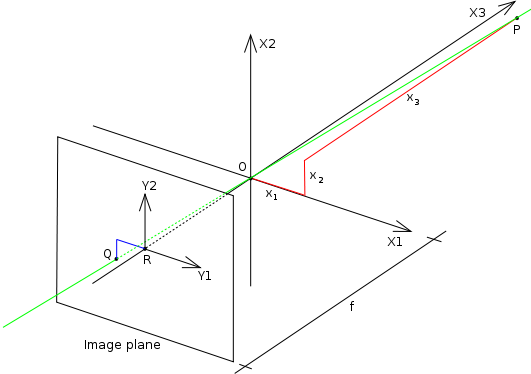
\includegraphics[width=5cm]{images/531px-Pinhole.png}
	\caption{Modelo de cámara Pin Hole. }
	\label{fig:Pin-Hole}
\end{figure}

La figura  [\ref{fig:Pin-Hole}] muestra los principales elementos que componen el modelo: 


\begin{enumerate}
	\item Un sistema de coordenadas 3D con origen en 0. Los 3 ejes del sistema de coordenadas son referidos como X1, X2 y X3. El eje X3 apunta en dirección a la camara y es referencia como el eje óptico o eje principal. El plano que intersecciona con los ejes X1 y X2 (plano principal) se encuentra en frente de la cámara.
	
	\item El plano de la imagen donde el mundo 3D se proyecta en dirección al centro óptico. Siendo éste paralelo a los ejes X1 y X2 localizados a una distancia "f" desde el origen O en la dirección negativa del eje X3. Dicha distancia es conocida como la distancia focal.
	
	\item Un punto R en la intersección del eje óptico y el plano de la imagen. Este punto es reperido como el punto principal o el centro de la imagen.

	\item Un punto P en algún lugar del entorno con coordenadas($x_{1}$,$x_{2}$,$x_{3}$).
	
	\item La línea de proyección del punto P a la cámara.
	
	\item La proyección del punto P al plano de la imagen, denotado como Q Este punto es dado por la intersección del la línea de proyección(verde) y el plano de la imagen.
	
	\item Finalmente, hay un sistema de coordenadas 2D en el plano de la imagen, con origen R y con los ejes Y1 y Y2 que son paralelos a X1 y X2, respectivamente.
\end{enumerate}

A pesar del pequeño tamaño de las lentes, las imágenes captadas no son perfectas. Existen pequeñas deformaciones que no son apreciables para el ojo humano, por lo que obtener los parámetros intrínsecos de la cámara juega un papel esencial en cada uno de los algoritmos para obtener unas medidas correctas. La obtención de dichos parámetros recibe el nombre de calibración, calculando la matriz de calibración K [\ref{eq:matrizK}].


\begin{equation}\label{eq:matrizK}
K=
\begin{pmatrix}
f_{x} & 0 & u_{0} \\
0 & f_{y} & v_{0} \\
0 & 0 & 1
\end{pmatrix}
\end{equation}

Los parámetros $f_{x}$ y $f_{y}$ representan la distancia focal en los ejes X e Y, mientras que $u_{0}$ y $v_{0}$ la posición del centro óptico en la imagen. Esta matriz permite realizar la proyección de un punto 3D en el mundo a un punto 2D en el plano
imagen de nuestra cámara, sólamente necesitamos multiplicar dicho punto por la matriz K.


\begin{equation}\label{eq:proyection}
\begin{pmatrix}
u\\
v\\
1
\end{pmatrix}=\begin{pmatrix}
f_{x} & 0 & u_{0} \\
0 & f_{y} & v_{0} \\
0 & 0 & 1
\end{pmatrix}\cdot\begin{pmatrix}
x\\
y\\
z \\
1
\end{pmatrix}
\end{equation}



Ahora bien la localización 3D o pose se define como la posición 3D de la cámara y su orientación respecto cierto sistema de referencia externo, y se suele expresar como una matriz 3x4 (4x4 si trabajamos en coordenadas homogéneas) que es el resultado de la multiplicación entre una matriz de rotación (R) 3x3 por un vector de traslación (t) 3x1.

\begin{equation}\label{eq:matrizRT}
RT=\begin{pmatrix}
r_{11} & r_{12} & r_{13} \\
r_{21} & r_{22} & r_{23} \\
r_{31} & r_{32} & r_{33}
\end{pmatrix}\cdot \begin{pmatrix}
t_{x}\\
t_{y}\\
t_{z}
\end{pmatrix}
\end{equation}

Quedando la proyección finalmente como:

\begin{equation}\label{eq:ProyectionDef}
P_{uv}=K\cdot RT\cdot P_{XYZ}
\end{equation}







\subsubsection{Perspective-n-Point}
Una vez explicado como se proyectan los puntos del mundo 3D al plano 2D de una cámara, 
podemos pasar al calculo de la localización de la cámara dado un conjunto \textit{n} de puntos 3D y sus proyecciones 2D. Dicho problema fue presentado por Fischler y Bolles \cite{Fischler}, denotándolo como Perspective-n-Point [\ref{fig:PnP}]:

\begin{figure}[H]
	\centering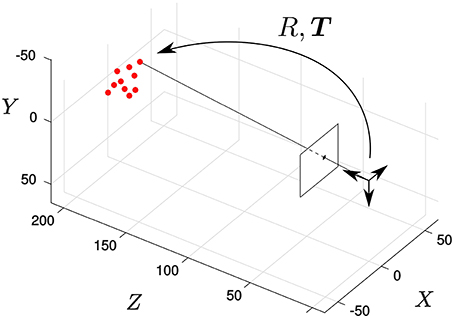
\includegraphics[width=5cm]{images/perspective_n_point.jpg}
	\caption{Perspective-n-Point}
	\label{fig:PnP}
\end{figure}

Dependiendo de la cantidad de puntos que tengamos existen varias soluciones:

\begin{itemize}
	\item Dos puntos o menos: soluciones infinitas.
	\item Tres puntos: ocho posibles soluciones de las cuales, la mitad están frente a la cámara (Haralick et 	al., 1994 \cite{trespuntos}).
	\item Cuatro puntos: si los cuatro puntos son coplanares solo existe una solución, en cualquier otro caso hay dos soluciones [Horaud et al., 1989 \cite{cuatropuntos}].
	\item Cinco puntos: es posible encontrar una solución pero ésta dependerá del método que utilicemos para minimizar el error. La técnica más usada es la de los mínimos cuadrados, pero también existen otras con una mejor eficiencia y precisión \cite{cincopuntos}.
\end{itemize}





%-------------------------------------------------------------------------
\section{Localización sin mapa conocido}


En la anterior sección he explicado algunos de los algoritmos del estado del arte para los casos en los que poseemos un mapa, con una serie de puntos conocidos XYZ que se proyectarán en la cámara y a través de algoritmos como Perspective-n-Point podemos averiguar la posición y orientación del sensor.



En esta sección explicaré algunos de los algoritmos más famosos en el caso de que no tengamos un mapa.

\subsection{Odometría visual}

La odometría visual es el proceso de determinar la posición y la orientación del sensor analizando una secuencia de imágenes captadas por la cámara. La odometría es un término que se utiliza generalmente en el campo de la robótica en el que se estima la posición del robot con ruedas durante la navegación. Para poder estimarla se usa la información sobre la rotación de las ruedas.

Por otro lado, el término "odometría visual" ,fue acuñado por Nister \cite{odometriavisual}, no requiere conocer la geometría del robot, se puede usar en cualquier robot que incorpore una cámara.

Dependiendo del tipo de visión que presente el robot, la odometría visual se basará en diferentes métodos.

\subsubsection{Odometría visual con visión monocular}
La utilización de una sola cámara para localizarte implica una mayor complejidad que en el problema de visión estéreo. Debemos tomar una serie de imágenes separados a una cierta distancia, y emparejar aquellos puntos de interés. Además si queremos conocer la escala real de la escena debemos conocer las medidas de algunos de los objetos presentes en el entorno.

Los algoritmos que hacen uso de la visión monocular se podrían clasificar de la siguiente forma:
\begin{itemize}
	\item Basados en características: buscan puntos característicos en la escena y realiza un seguimiento de éstos. El movimiento de la cámara se obtiene minimizando el error de reproyección de los puntos emparejados, utilizando algoritmos iterativos de optimización.
	
	El punto de fuerte de estos métodos se encuentra en que existen algoritmos de detección de puntos de interés bastante robustos, pero por contra dependerá mucho de los umbrales que se impongan y su precisión puede verse afectada por emparejamientos incorrectos.

	\item Métodos directos: en lugar de buscar de puntos característicos, utiliza la información de la intensidad de los píxeles para determinar el movimiento del sensor.
	
	Estos métodos funcionaran mejor en aquellas situaciones en las que el fondo no posea mucha textura (es más díficil buscar esquinas) y, además el tiempo de cálculo se verá reducido ya que no se tiene que extraer puntos y calcular sus emparejamientos.
	
	\item Métodos híbridos: son métodos que combinan ambos sistemas.
\end{itemize}

\subsubsection{Odometría visual con visión estéreo}
Los algoritmos en la visión estéreo son similares a los explicados en la visión monocular, con la diferencia de que ahora tenemos dos cámaras que toman imágenes de forma simultánea y que
comparten una parte de su campo de visión.

La principal ventaja que tiene esta odometría es que al poseer dos cámaras podemos estimar la profundidad a la que se encuentra los objetos mediante geometría epipolar[\ref{fig:epipolar}].
\begin{figure}[H]
	\centering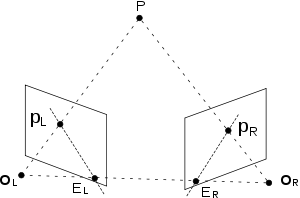
\includegraphics[width=6cm]{images/epipolar.png}
	\caption{Modelo de cámara Pin Hole. }
	\label{fig:epipolar}
\end{figure}
Esta odometría visual se ha utilizado en el campo de la robótica tanto para la navegación [referencia] como para algoritmos SLAM

\subsection{SLAM}
Los algoritmos conocidos como SLAM (\textit{Simultaneous Localization and Mapping}) son aquellos capaces de generar un mapa y localizar al sensor de forma simultánea. Estos algoritmos se han utilizado en el campo de la robótica típicamente con láseres, sónares o cámaras estéreos pero con el paso del tiempo se desarrollaron algoritmos que utilizasen un solo sensor.

\subsubsection{Mono-SLAM}
El término Mono-SLAM hace referencia al uso de una sola cámara para RGB para la localización y creación de un mapa de forma simultánea. El primero que propuso el uso de una única cámara Andrew Davison a partir del año 2002 \cite{Davison07monoslam:real-time}.

Éste se encuentra basado en el uso de un filtro extendido de Kalman (EKF) para estimar la posición y orientación 3D de la cámara, así como la posición de una serie de puntos 3D que conforman el mapa. Para calcular la posición inicial de la cámara es necesario dotar al filtro de información a priori con la posición 3D de al menos cuatro puntos. Una vez estimada la posición, el algoritmo es capaz de situar la cámara 3D y de generar nuevos puntos del mapa que sirven como apoyo a la propia localización de la cámara.


\paragraph{Filtro kalman extendido}

El vector de estado del EKF se compone de la posición 3D de la cámara, su velocidad lineal, la rotación y su velocidad angular. Por otra parte, el modelo de transición actualiza el estado de la cámara aplicando un modelo de velocidad constante a la posición y orientación de la cámara teniendo en cuenta las velocidades lineal y angular de la iteración anterior.

Además el modelo de observación se compone de las proyecciones de cada uno de los puntos 3D en el plano imagen teniendo en cuenta la posición y orientación de la cámara.

\subsubsection{PTAM}
\label{sec:PTAM}
El algoritmo PTAM (\textit{Parallel Tracking and Mapping}) ,escrito por Georg Klein y David Murray \cite{klein07parallel},pretende solucionar los problemas que tiene el algoritmo de MonoSLAM pero desde un punto de vista totalmente diferente. MonoSLAM estima y actualiza su localización a través de un filtro de Kalman extendido, mientras que PTAM utiliza métodos de optimización.

El principal problema del algoritmo de MonoSLAM es que su tiempo de ejecución aumenta exponencialmente con el número de puntos del mapa. Esto se debe a que en cada iteración, se actualiza la posición de cada objeto del mapa y la localización de la cámara. 

PTAM parte de la premisa que el hilo de tracking debe ejecutarse en tiempo real, mientras que el del mapa no tiene por qué actualizarse en cada iteración. 

\paragraph{Tracking}
El hilo del tracking sigue los siguientes pasos:
\begin{enumerate}
	\item Preprocesado de las imágenes: La imagen se divide en 4 subimágenes de distinta resolución y se buscan puntos característicos con el algoritmo FAST de Rosten, Edward y Drummond, Tom \cite{Rosten:2006}.
	\item Actualización de la posición con modelo de movimiento: A continuación se actualiza la posición con un modelo de velocidad constante[\ref{eq:vel_cte}], como se muestra a continuación:
	\begin{equation}\label{eq:vel_cte}
	v_{t}=\frac{x_{t}-x_{t-1}}{\Delta t}
	\end{equation}
	\item Actualización de grano grueso: se seleccionan una número \textit{n} de puntos 3D del mapan y se proyectan en la cámara. A continuación se realiza un emparejamiento comparando parches alrededor de los píxeles que se han proyectado. Una vez que se encuentren emparejados se minimiza el error de proyección a través del proceso de optimización de Gauss-Newton Kelley \cite{Gauss-Newton}
	\item Actualización de grano fino: En esta ocasión se toman hasta mil puntos del mapa y se sigue el mismo procedimiento que en el paso anterior. Al tomar un mayor número de puntos se obtiene una estimación con mayor precisión.

\end{enumerate}
\paragraph{Mapping}
Por otro lado, el hilo del \textit{Mapping} debe inicializarse primero para su correcto funcionamiento. Ésta se realiza con el seguimiento de una serie de imágenes tomadas a un cierta distancia, emparejando puntos característicos y calculando su posición con el algoritmo de cinco puntos. Cabe decir que el mapa que se creará puede no tener una posición 3D totalmente real, pero representa la realidad a una escala diferente.

Dicho hilo sigue los siguientes pasos:
\begin{enumerate}
	\item Añadir nuevos Keyframes: no todos los frames son utilizados para procesarlos ya que supondría una gran carga computacional y ,además, puede que contengan información redudante. Por ello, sólo se añadirán si cumplen una serie de condiciones: que el tiempo entre Keyframe y Keyframe supere un cierto valor, que su distancia sea adecuada, y que la estimación de la posición sea bueana.
	\item Añadir nuevos puntos 3D al mapa: una vez añadido el \textit{Keyframe} al mapa, se calcula una serie de puntos característicos y se buscan en anteriores Keyframes. Los puntos emparajedos se añaden al mapa, calculando su posición mediante triangulación. Dichos puntos son los que se proyectarán en el hilo de \textit{tracking}.
	\item Optimizar el mapa: Si el hilo del mapa se encuentra libre, se refina la posición 3D de los puntos guardados mediante el algoritmo de \textit{Bundle Adjustment} con el fin de minimizar el error de proyección entre \textit{m} posiciones en 3D de la cámara y \textit{n} puntos 3D.
	
	
	\item Mantenimiento del mapa: Finalmente, se elimina aquellas asociaciones de puntos mal realizadas y añadiendo nuevos puntos cuando sea posible.
	
\end{enumerate}

El principal problema que posee el algoritmo de PTAM es que como el título de su paper dice sólo se puede utilizar en pequeñas zonas de trabajo. El numero de puntos que debe procesar crece con bastante rapidez provocando un mayor tiempo de cálculo.

\paragraph{Comparativa entre MonoSLAM y PTAM: } El autor del paper intenta comparar su algoritmo con otros(EKF-SLAM), en un seguimiento de una trayectoria. Como podemos ver en la figura [\ref{fig:PTAM}] el algoritmo PTAM ofrece una trayectoria con más precisa.

\begin{figure}[H]
	\centering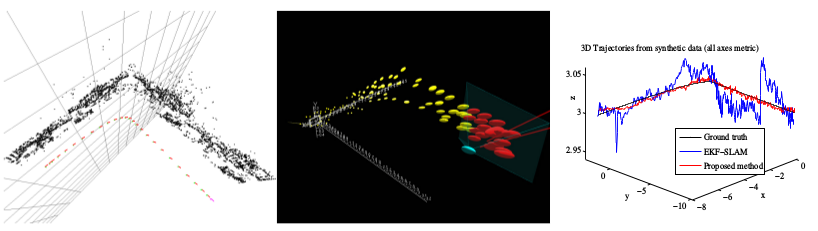
\includegraphics[width=12cm]{images/PTAM.png}
	\caption{Comparativa entre MonoSLAM y PTAM: La imagen de la izquierda muestra el mapa creado por PTAM, mientras que la segunda muestra el mapa creado por EKF-SLAM.}
	\label{fig:PTAM}
\end{figure}


\subsubsection{DTAM}
DTAM (\textit{Dense Tracking and Mapping}) escrito por A. Newcombe et al. en el 2011 \cite{DTAM} aborda el problema del SLAM monocular usando la información de todos los píxeles en lugar de puntos caracterísiticos. Al utilizar toda la información de la imagen se consigue un mapa denso de la escena que conllevará una gran carga computacional.

Los autores del paper hacen hincapié DTAM es capaz de trabajar en tiempo real en equipos potentes debido a que el algoritmo es paralelizable y permite su ejecución en GPU.

\paragraph{Tracking}
En primer lugar,la inicialización de la pose se realiza de una manera similar que el algoritmo de PTAM [\ref{sec:PTAM}] (actualización de grano grueso y fino) pero en lugar de minimizar el error de reproyección se minimiza el error fotométrico.
\paragraph{Mapping}

El hilo del \textit{mapping} se ocupa de la generación del mapa mediante el uso de varias vistas. El proceso de reconstrucción se realiza con todos los fotogramas de entrada, y mediante un proceso que pretende reducir la energía de la imagen se refina la generación del mapa.


\paragraph{Comparativa entre PTAM y DTAM} DTAM ofrece unos resultados mas satisfactorios a la hora del tracking que el algoritmo de PTAM debido al mapa denso. El autor del paper lo intenta demostrar siguiendo a un objeto (taza) y agitando la cámara. Como podemos ver en la figura [\ref{fig:DTAM}] en los momentos en los que agita la cámara (a partir del frame 1000) el algoritmo PTAM pierde la taza.
\begin{figure}[H]
	\centering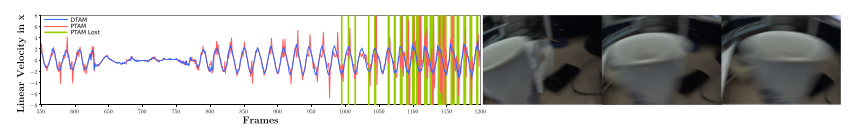
\includegraphics[width=12cm]{images/DTAM.png}
	\caption{Comparativa entre PTAM y DTAM. La primera grafica muestra como evoluciona el seguimiento de la taza a lo largo de los frames. La segunda imagen muestra como agita la cámara distorsionando la imagen}
	\label{fig:DTAM}
\end{figure}
\subsubsection{ORB-SLAM}
El algoritmo ORB-SLAM \cite{ORB-SLAM} escrito por Mur-Artal, R. y Montiel, J.M.M. y Tardos, J.D, es un algoritmo SLAM basado en la búsqueda de puntos característicos que puede funcionar con visión monocular, visión estéreo y con sensores RGBD. Su peculiaridad se encuentra en el uso del descriptor ORB \cite{ORB-descriptor} para encontrar los puntos de interés y un modelo de bolsa de palabras \cite{bolsa}  para detectar cierres de bucle y, en su caso, para relocalizarse.

A diferencia de los SLAM explicados, éste posee un hilo más que se usa para detectar cierres de bucle: \textit{looping}
\paragraph{Tracking}
Al igual que en otros algoritmos se estima su posición mediante el uso de un modelo de movimiento emparejando los puntos 3D visibles en el fotograma anterior, calculando la posición actual a partir de
los emparejamientos realizados.

Pero en esta ocasión si el robot se pierde se utiliza un modelo de bolsa de palabras para obtener Keyframes candidatos que concuerden con la observación actual.
\paragraph{Mapping}
La inicialización del mapa se realiza calculando en paralelo un mapa por homografía y otro mediante una matriz fundamental. Ambos modelos obtienen una puntuación para determinar cuál será el utilizado para inicializar el mapa, de forma que en aquellas escenas que cuenten con un plano principal se utilizará la homografía y en el resto de los casos se utilizará la matriz fundamental.



Otra caracterítica de este algoritmo es que genera un grafo donde los vértices se corresponden con Keyframes y las aristas entre vértices se generan siempre que los Keyframes tengan varios puntos 3D en común. Este grafo se utiliza entre otras cosas para eliminar Keyframes redundantes
\paragraph{Looping}
Finalmente el hilo \textit{Looping} se encarga de comprobar si se ha producido un cierre de bucle. Para ello. utiliza el grafo de Keyframes conectados y el modelo de bolsa de palabras, con el objetivo de buscar Keyframes candidatos con apariencia similar a la observación actual.
\bibliography{egbib}






\end{document}
